\section{Physics Background}

\subsection{Resonant Cavities}
We begin our discussion with a description of the physics problem at hand, as well as a derivation for the mathematics used. Implicitly in the title of this project we are looking at \emph{resonant cavities}, which are volumes used to store standing waves. In the case of Electromagnetic waves that means that the walls of this cavity are perfect conductors. Most physics students will be able to draw parallels to a vibrating string as it is a common wave PDE problem. A one dimensional parallel for electromagnetic waves would be two parallel mirrors separated by a distance L. In this case, the normal modes are electromagnetic waves that bounce between the mirrors such that the total trip is an integer number over wavelengths\cite{Zangwill}. This would be analogous to the \emph{standing wave} on the string where the nodes and antinodes are stationary.

The approach we will use to find the standing waves of a conducting cavity focuses on time-harmonic and divergence-free solutions of the homogeneous wave equation in a volume $V$ with surface $S$\footnote{At this point I am showing my future aspirations of being a theorist by using natural units $c=\hbar=1$. This should make little difference to the physics we are studying, and it makes the equations slightly nicer.}.
\ea{
\qty(\laplacian + \epsilon\mu\omega^2)\va{E} &= 0 \ \text{ in V} \label{eq:Helmholtz}\\
\div \va{E} &= 0 \ \text{ in V}\\
\value{n} \cross \va{E} &= 0 \ \text{ on S}
}
Here $\epsilon$ is the electric permutivity of the volume, $\mu$ is the magnetic permutivity, and $\va{E}$ is the electric field which has the following spacial and temporal components:
\eq{
\va{E} = \va{E}(\va{r})e^{-i\omega t}
}
Solving the Helmholtz equation \eqref{eq:Helmholtz} is analytically possible for simple geometries using separation of variables. These geometries include variations on cylinders, rectangular prisms, and spheres. For further reading on the solutions to the Helmholtz equation you are welcome to suffer like every other Physics graduate student and read \cite{Jackson}.

\subsection{Derivation for a Spherical Cavity}
Armed with a deeper understanding of resonant cavities, we can now turn our attention to the problem at hand, spherical cavities. The electromagnetic normal modes of a spherical resonant cavity are time-harmonic, vector spherical waves that satisfy the perfect-conductor boundary condition $\vu{r}\cross \va{E}\big{|}_s=0$ at the cavity’s walls \cite{Zangwill}. If we take $u(r,\theta,\phi)$ to be the solution to \eqref{eq:Helmholtz} then our normal modes would take the form of transverse magnetic and transverse electric waves.
\ea{
\va{E}_E = -i\omega\va{r}\cross\grad u &\hlw{.05} \va{E}_M = \curl(\va{r}\cross\grad u)\\
\va{B}_E = -\curl(\va{r}\cross \grad u) &\hlw{.05} \va{B}_M = -i\omega\va{r}\cross\grad u
}
Most readers will find a parallel to other areas of Electrodynamics in that our solution to the Helmholtz equation will be a linear combinations of radial equations multiplying the spherical harmonics. In this case our radial function will be a combination of spherical Bessel functions ($j_l(kr)$) and spherical Neumann functions ($n_l(kr)$.
\eq{
u(\va{r}) = \sum_{lm}\qty(A_l j_l(kr) + B_l n_l(kr))Y_{lm}(\theta,\phi)
}
Here $k=\frac{\omega}{c}$. It will be related to the zeros of these Bessel functions, which is how we will obtain our Eigenvalues or Eigenfrequencies. In this case we are only concerned with behavior inside the cavity. Since $n_l$ diverges are the origin we are able to force all $B_l$ to be zero\cite{Jackson}. Thus the form of $u$ inside the cavity is the following:
\eqb{
u_{lm}(\va{r}) = A_l j_l(kr))Y_{lm}(\theta,\phi)
}
Computing the various transverse waves above will require some vector calculations on this solution. The following identity will prove to be quite useful due to the nature of spherical harmonics.
\eq{
\curl(\va{r}\cross\grad u) = \va{r}\laplacian u - 2\grad u - r\pdv{r}\grad u
}
This allows us to write the form of the transverse electric and magnetic waves\cite{Zangwill}.
\ea{
E_E &= i\omega j_l(kr)\qty(\frac{1}{\sin\theta}\pdv{Y_{lm}}{\phi}\vu{\theta}-\pdv{Y_{lm}}{\theta}\vu{\phi}) \label{eq:wave1}\\
\nonumber\\
E_M &= -\qty(\frac{l(l+1)}{r^2}\va{r}+\qty[\vu{\theta}\pdv{\theta}+\vu{\phi}\frac{1}{\sin\theta}\pdv{\phi}]\frac{1}{r}\pdv{r})rj_l(kr)Y_{lm}(\theta,\phi) \label{eq:wave2}
}

\subsection{Analytic Solutions}

In order to make sure that we have a complete understanding of the Bessel functions we will do a slight review. Bessel functions are the solutions to Bessel's differential equation:
\eq{
x^2\dv[2]{y}{x} + x\dv{y}{x}+(x^2-m^2)y = 0
}
Most readers will be familiar with the form of cylindrical Bessel functions as the solution to the Laplace equation in cylindrical coordinates. These functions occur in the case where $m$ is an integer value. The solutions to the Helmholtz equation are the spherical Bessel functions. These functions occur when $m$ is a half integer. In such a case we make the transformation $m^2\to l(l+1)$ so that $l$ can be used as an integer index for the functions. It is customary to represent spherical Bessel functions will lowercase letters and cylindrical Bessel functions with uppercase\cite{handbook}. While these functions can be related to cylindrical Bessel functions, they are unique with respect to the fact that there is a much simpler way of writing them. Specifically we will use Rayleigh's formulas and then push forward.
\ea{
j_l(x) &= (-1)^l \qty(\dv{x})^l\frac{\sin(x)}{x}\\
n_l(x) &= (-1)^l+1 \qty(\dv{x})^l\frac{\cos(x)}{x}\\
}
\begin{figure}
    \centering
    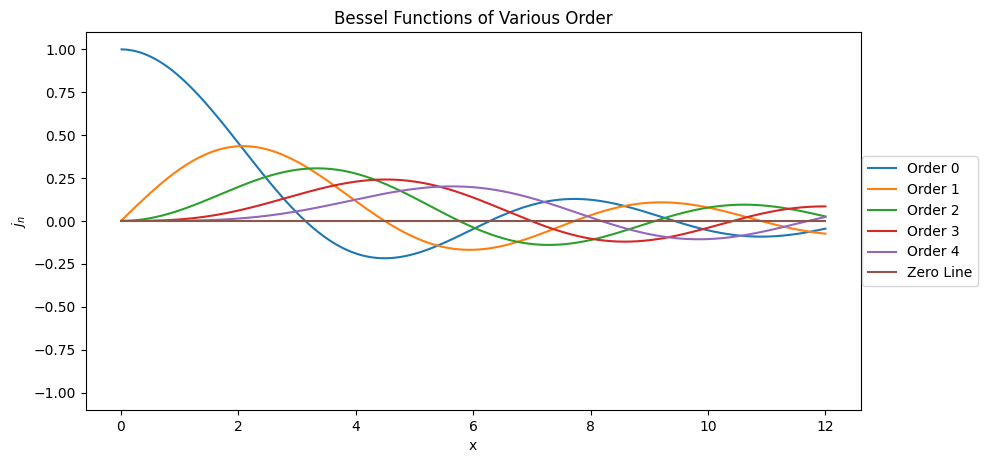
\includegraphics[width=.8\linewidth]{Bessel.png}
    \caption{Spherical Bessel functions of various order}
    \label{fig:bessel}
\end{figure}
While we could go down an endless rabbit hole when it comes to Bessel functions, I believe this will be enough for the problem at hand.

We're most interested in finding the Eigenfrequencies of the spherical cavity. To do so we look back at the boundary condition $\vu{r}\cross \va{E}\big{|}_s=0$. When applied to equations \eqref{eq:wave1} and \eqref{eq:wave2} this means that the angular comonents of those waves must be zero for any value all values of $\theta$ and $\phi$ when $r=R$ (the outer radius of the vanity). The only way to do so is to set either the Bessel function of the derivative of the Bessel function to zero at the walls.
\ea{
j_l(k_{n,l}R) &= 0\\
\dv{r}\qty(rj_l(k_{n,l}r))\big{|}_{r=R} &= 0 \label{eq:annoying}
}
%The magnetic wave equation requires us to make use of the derivative relation
%\eq{\qty(\frac{1}{z}\dv{z})^m \qty(z^{l+1}J_l(z)) = z^{l-m+1}J_{l-m}(z)}
%Thus simplifying equation \eqref{eq:annoying} to the following:
%\eq{\dv{r}\qty(rj_l(kr)) = \frac{1}{k}\dv{kr}\qty(rj_l(kr))}

This allows us to write down the Eigenfrequencies in terms of the zeros of the bessel functions ($x_n,l)$.
\eqb{
\omega = x_{n,l}\frac{c}{R}
}
The zeros have multiple frequencies as the zeros of the $l$ bessel function are not the same as the zeros of the $l+1$ function. Moreover, due to the periodic nature of $\sin$ and $\cos$ each order of Bessel function has many zeros.

At this point it is clear that our goal is calculate the zeros of the various Bessel functions. Doing so by hand is rather straight forward, but it takes time, especially for higher order Bessel functions. Since these functions have been around for so long most people consult a table of zeros when they are needed. In our case

\section{Computational Solutions}
%Be sure to mention what you are using and why
During lecture we looked at multiple methods for root finding numerically. These methods have a direct parallel to a sort of graphical search in that they were easy to animate. Specifically we looked at four methods:
\begin{enumerate}
    \item Simple Search: Where we took a midpoint of a specific range and cut the step size in half each iteration
    \item Bisection: This method utilizes the intermediate value theorem to find one root in a given interval
    \item Secant Line: Draws a line connecting two points and uses the intersection at zero to start the next integration.
    \item Utilizes the derivative of the function to draw a tangent line to begin next iteration.
\end{enumerate}
Since our Bessel functions are analytic the tangent method should be the most efficient. The scipy library holds Bessel functions and derivatives of Bessel functions for integer and half integer values. I used that alon with the algorithms mentioned in class to design my implementation.

Comparing these methods proved that assumption correct. We were also able to animate the search to more intuitively see how accurate they were. In general, even the simple search eventually hit the desired accuracy of $\pm 1\cross 10^{-6}$ within the max iterations.
\begin{figure}
    \centering
    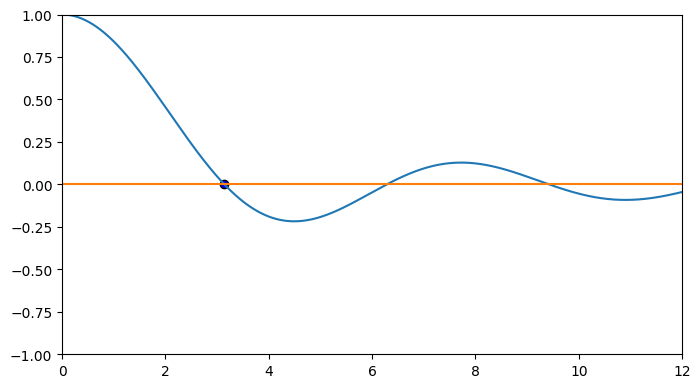
\includegraphics[width=.7\linewidth]{simple.png}
    \caption{The final plot of the simple search's attempt to find a zero of a Bessel function of the first kind}
    \label{fig:simple}
\end{figure}

While the animations may look nice I have a larger issue at hand. There are different algorithms in existence that can calculate the zeros of spherical Bessel functions quite exactly using the relation to cylindrical Bessel functions. In particular I think of the \href{https://scipy-cookbook.readthedocs.io/items/SphericalBesselZeros.html}{provided link} as my direct competition. This method also makes use of an algorithm that is able to use the previous zero to calculate the next one. Ideally I would like to be able to do something that these methods can't do.

These methods do have one fatal flaw, they require you to calculate every zero previous to the one that you are looking for. Since our method is more \emph{graphical} than a series, I do not have the same restraint. The hard part I need to overcome is I need a way to estimate a start point for my tangent search. 

If we ignore the area right around zero (\emph{I'll never beat the other algorithms at that small of a value of x anyway}) a spherical Bessel function of order 0 behaves like a $\sin$ function of decreasing amplitude.
\eq{
j_0 = \frac{\sin(x)}{x}
}
The zeros of a sin function are integer values of $\pi$ so I am already able to know exactly where these zeros are. Now if we look at a Bessel function of order 1 we essentially just subtract $\cos$.
\eq{
j_1 = \frac{1}{x}(\frac{\sin(x)}{x} - \cos(x))
}
Once again it is pretty easy to guess these roots, they occur at $z\pi-\frac{\pi}{2}$. At the risk of being too general I thought I could generalize this process. For a Bessel function of order $l$ the n-th zero should occur at:
\eqb{
\text{Estimated Zero } = (n+1)\pi-\frac{l\pi}{2}
}
Armed with this knowledge I might actually stand a chance against those other algorithms for higher values of $x$, which is the same as saying higher Eigenfrequencies. Testing this out when beautifully even at order 16 we were able to calculate the 30th root with only 7 iterations.\\
\\
Thus I believe I can make the following conclusion. Whilst it is more accurate to analytically calculate or use the series method \href{https://scipy-cookbook.readthedocs.io/items/SphericalBesselZeros.html}{outlined here} to calculate the zeros of spherical Bessel functions. Our iteration excels at higher orders and highers Eigenfrequencies. 

\section{Applications and Current Research}

Whilst I was searching for information on resonant cavities I came across some interesting research currently happening with regards to this topic. First I found \cite{research1} which used radial basis functions to solve the Helmholtz equation in rectangular coordinates as opposed to spherical ones. While I did not completely understand the math, the paper did have a very interesting visualization of the normal modes inside the chamber. I also found \cite{research2} which technically used an overall cylindrical geometry, however it did make use of perturbation theory which I found to be interesting.